\section{Introduction}
\label{sec:introduction}


Some general introduction to Monte Carlo methods and MCMC methods.

What are Monte Carlo and MCMC methods? What is the aim? What are the applications? A brief history? (Short comparison between numerical and stochastic methods? Advantages and disadvantages?)
\newline

1946, Los Alamos National Laboratory, New Mexico, U.S.A.. Mathematicians: John von Neumann, Stanislaw Ulam, Robert Richtmyer, Physicists: Enrico Fermi, Nick Metropolis, Edward Teller.
Invention of first electronic computers as ENIAC (Electronic Numerical Integrator And Computer) made it possible to simulate (Monte Carlo Simulation).

\subsection*{Statement of the problem}

Look at computational cost of MCMC methods as a function of dimension $ N $.

Optimal Scaling for RWM and MALA. 

\subsubsection*{Random Walk Metropolis algorithm}

In Figure \ref{fig:3DscatterplotRWM}, the opitimal scaling of the acceptance probability and therefore the scaling of the proposal variance is illustrated by a Random Walk Metropolis-Hastings algorithm. A too small proposal variance and therefore a too high acceptance probability causes a very slow mixing of the Markov chain in the two modes of the target density. In the case of a too high proposal variance, the Markov chain stays very long in one state. Hence the efficiency of the algorithm is relatively low.


\begin{figure}[htb]
 \begin{center} 
  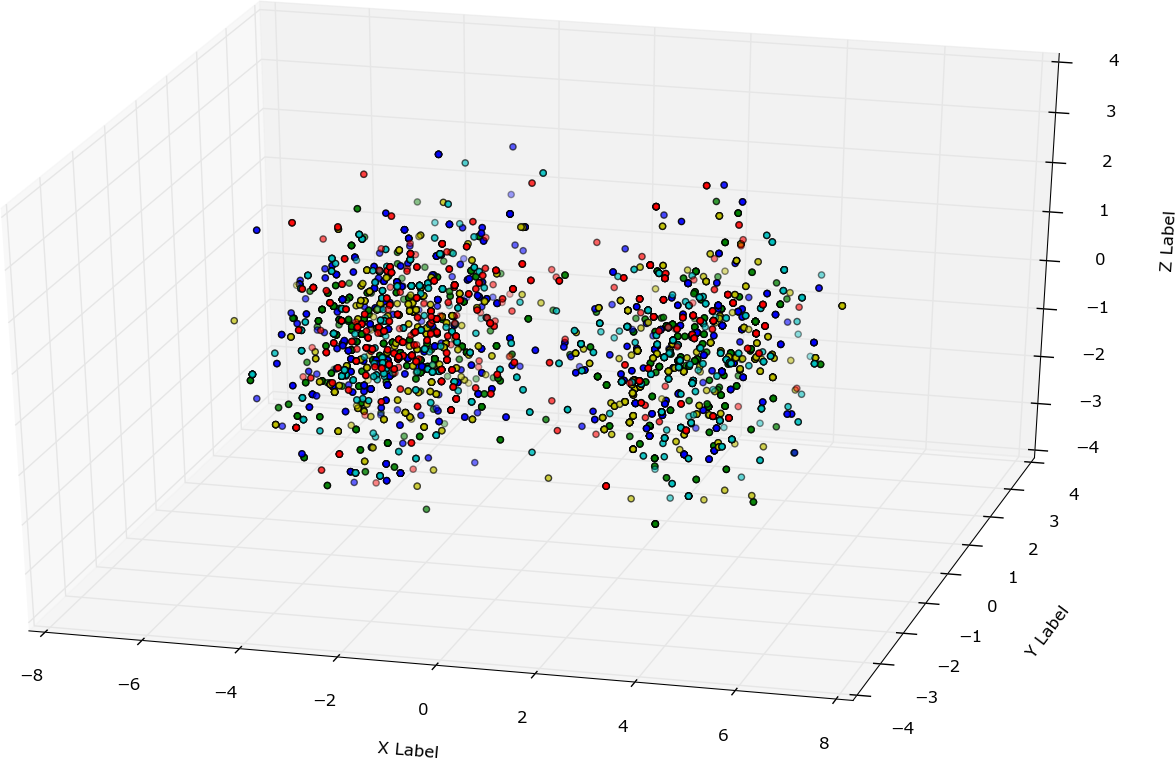
\includegraphics[width=0.69\textwidth]{figure_1}
  \vspace*{1mm}
  \subcaption{Optimal scaled acceptance probability with a good mixing between both modes.}
  \vspace*{3mm}
  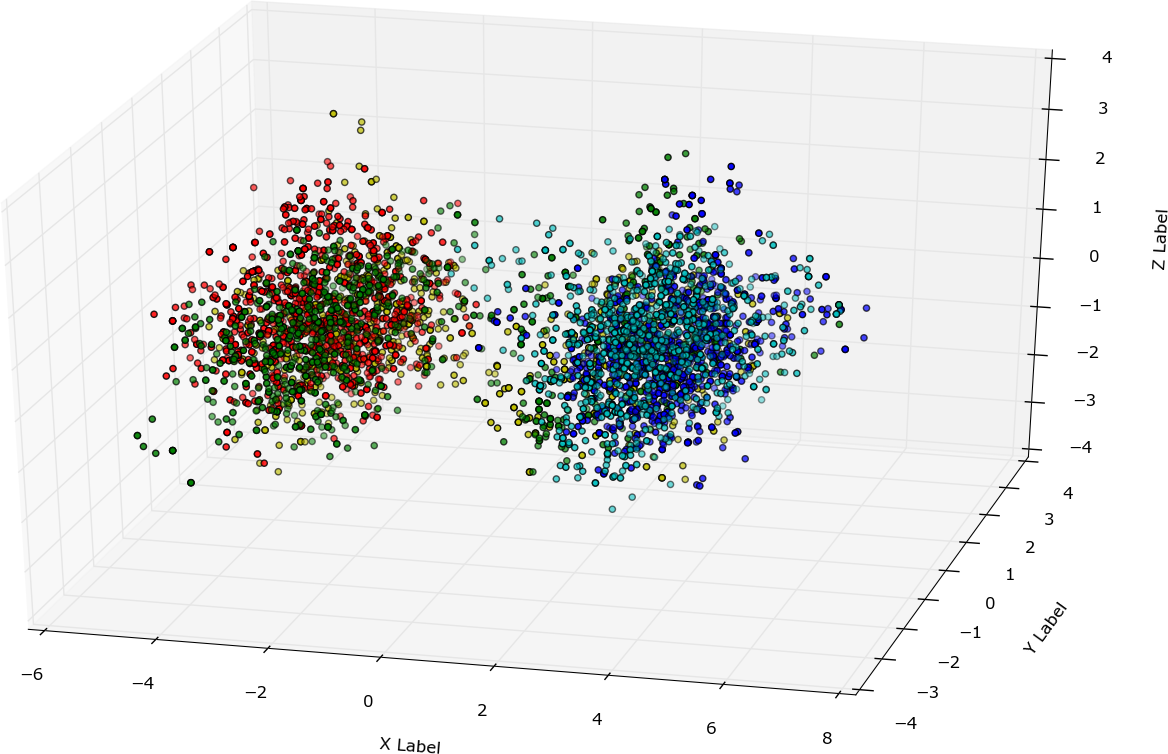
\includegraphics[width=0.69\textwidth]{figure_2}
  \vspace*{1mm}
  \subcaption{Too large acceptance probability with a bad mixing between both modes.}
  \vspace*{3mm}
  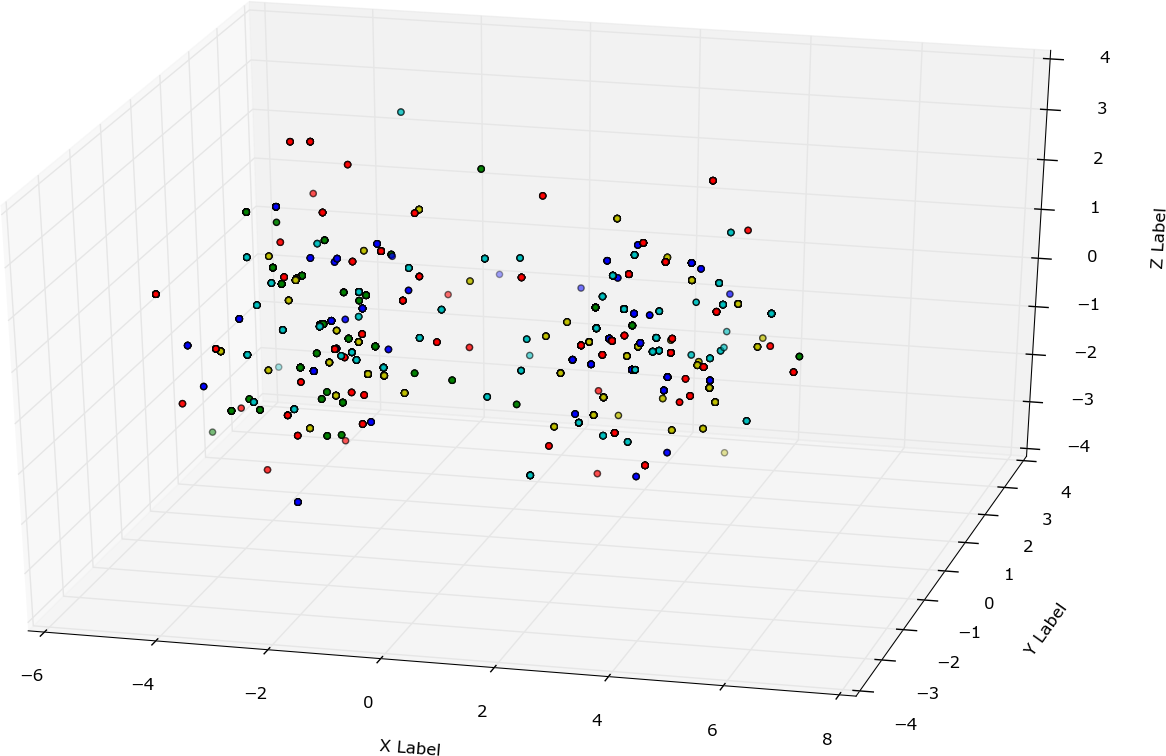
\includegraphics[width=0.69\textwidth]{figure_3}
  \vspace*{1mm}
  \subcaption{Too low acceptance probability.}
 \end{center}
  \caption{5000 samples produced by a RWM algorithm of a multimodal non-product target density. Every 1000 consecutive samples are labeled in the same colour.}
  \label{fig:3DscatterplotRWM}
\end{figure}

\subsection*{Own contributions}

My contributions to the present topic.
\begin{itemize}
 \item First point.
 \item Second point.
 \item Last point.
\end{itemize}


\subsection*{Outline}

A brief outline of the structure of this work.

Give an overview of present results of optimal scaling: Roberts and Rosental, Bedard, Breyer and Piccioni and Scarlatti, Mattingly and Pillai and Stuart and Thiery

\subsection*{Acknowledgements}

A list of persons, who deserve my acknowledgements: advisor, parents, friends.



